\documentclass[crop,tikz]{standalone}
\usepackage[none]{hyphenat}
\usepackage{helvet}
\renewcommand{\familydefault}{phv}

\makeatletter
\renewcommand{\large}{\@setfontsize\large{10}{9}}
\renewcommand{\normalsize}{\@setfontsize\normalsize{8}{9.5}}
\makeatother

\usepackage{tikz}

\begin{document}
\pagestyle{empty}

\definecolor{yellow}{rgb}{1.0, 1.0, 0.45} % 255/255/115
\definecolor{dkyellow}{rgb}{0.9, 0.9, 0.0} % % 230/230/0

\definecolor{ltorange}{rgb}{1.0, 0.74, 0.41} % 255/188/105
\definecolor{orange}{rgb}{0.96, 0.50, 0.0} % 246/127/0

\definecolor{ltred}{rgb}{1.0, 0.25, 0.25} % 255/64/64
\definecolor{red}{rgb}{0.79, 0.00, 0.01} % 201/0/3

\definecolor{ltpurple}{rgb}{0.81, 0.57, 1.00} % 206/145/255
\definecolor{purple}{rgb}{0.38, 0.00, 0.68} % 97/1/175

\definecolor{ltblue}{rgb}{0.2, 0.73, 1.0} % 51/187/255
\definecolor{blue}{rgb}{0.12, 0.43, 0.59} % 30/110/150

\definecolor{ltltgreen}{rgb}{0.7, 1.00, 0.7} % 96/204/14
\definecolor{ltgreen}{rgb}{0.37, 0.80, 0.05} % 96/204/14
\definecolor{green}{rgb}{0.23, 0.49, 0.03} % 59/125/8
  
\definecolor{dkslate}{rgb}{0.18, 0.21, 0.28} % 47/53/72
\definecolor{mdslate}{rgb}{0.45, 0.50, 0.68} % 114/127/173
\definecolor{ltslate}{rgb}{0.85, 0.88, 0.95} % 216/225/229

\pgfdeclarelayer{background}
\pgfsetlayers{background,main}


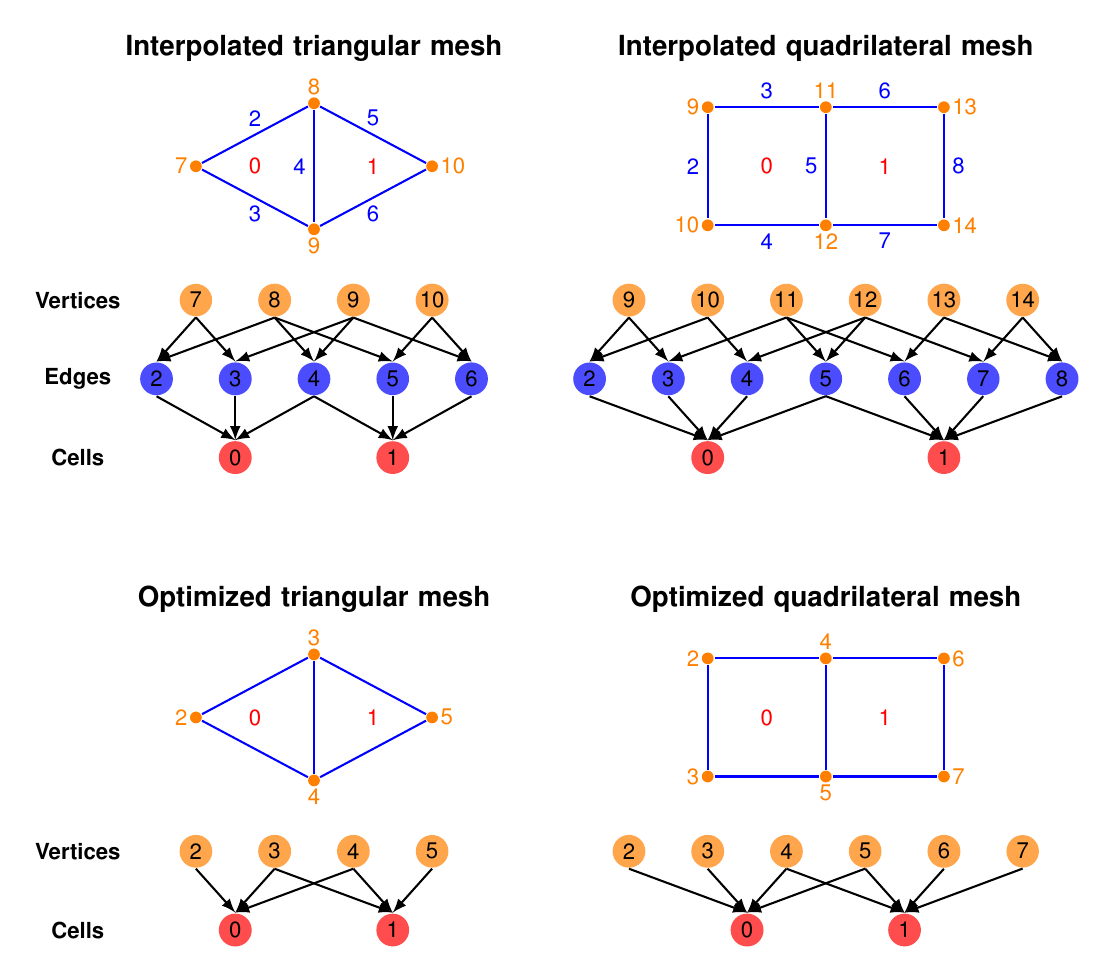
\begin{tikzpicture}[>=latex,line width=0.75pt]

\usetikzlibrary{shapes,calc}%

\colorlet{colvertex}{orange}
\colorlet{coledge}{blue}
\colorlet{colcell}{red}

\tikzstyle{title}=[text width=62mm,text centered,font=\bfseries\large]
\tikzstyle{annotate}=[font=\bfseries]

\tikzstyle{vertex}=[circle,color=black,fill=colvertex,inner sep=1.5pt]
\tikzstyle{vlabel}=[color=colvertex]

\tikzstyle{edge}=[color=coledge,line width=0.75pt]

\tikzstyle{tri}=[color=colcell,regular polygon,regular polygon sides=3,line width=0.5pt]
\tikzstyle{quad}=[color=colcell,regular polygon,regular polygon sides=4,line width=0.5pt]

\tikzstyle{gpoint}=[circle,color=black,text centered,text width=1.3em,inner sep=0pt]
\tikzstyle{gvertex}=[gpoint,fill=colvertex!70]
\tikzstyle{gedge}=[gpoint,fill=coledge!70]
\tikzstyle{gcell}=[gpoint,fill=colcell!70]

% Reference points
\coordinate (o1) at (-70mm,0mm);
\coordinate (o2) at (-5mm,0mm);
\coordinate (o3) at (-70mm,-70mm);
\coordinate (o4) at (-5mm,-70mm);


% ----------------------------------------------------------------------
% Interpolated tri mesh

\node[title] at ($ (o1)+(0,15mm) $) {Interpolated triangular mesh};

% Vertices
\node[vertex] (a_p7) at ($ (o1)+(-15mm,+0mm) $) {}; \node[vlabel,left] at (a_p7) {7};
\node[vertex] (a_p8) at ($ (o1)+(0mm,+8mm) $) {}; \node[vlabel,above] at (a_p8) {8};
\node[vertex] (a_p9) at ($ (o1)+(0mm,-8mm) $) {}; \node[vlabel,below] at (a_p9) {9};
\node[vertex] (a_p10) at ($ (o1)+(+15mm,0mm) $) {}; \node[vlabel,right] at (a_p10) {10};

% Edges
\path[edge] (a_p7) edge node[above] {2} (a_p8);
\path[edge] (a_p7) edge node[below] {3} (a_p9);
\path[edge] (a_p8) edge node[left] {4} (a_p9);
\path[edge] (a_p8) edge node[above] {5} (a_p10);
\path[edge] (a_p9) edge node[below] {6} (a_p10);

% Cells
\node[tri] at ($ (o1)+(-7.5mm,+0mm) $)  {0};
\node[tri] at ($ (o1)+(+7.5mm,+0mm) $)  {1};

% Graph
\node[annotate] (a_v) at ($ (o1)-(30mm,17mm) $) {Vertices};
\node[annotate,below of=a_v] (a_e) {Edges};
\node[annotate,below of=a_e] (a_c) {Cells};

% Vertices
\node[gvertex,right of=a_v,xshift=5mm] (a_g7) {7};
\node[gvertex,right of=a_g7] (a_g8) {8};
\node[gvertex,right of=a_g8] (a_g9) {9};
\node[gvertex,right of=a_g9] (a_g10) {10};

% Edges
\node[gedge,below of=a_g7,xshift=-5mm] (a_g2) {2};
\node[gedge,right of=a_g2] (a_g3) {3};
\node[gedge,right of=a_g3] (a_g4) {4};
\node[gedge,right of=a_g4] (a_g5) {5};
\node[gedge,right of=a_g5] (a_g6) {6};

% Cells
\node[gcell,below of=a_g3] (a_g0) {0};
\node[gcell,below of=a_g5] (a_g1) {1};

% connections
\draw[->] (a_g7.south) -- (a_g2.north);
\draw[->] (a_g7.south) -- (a_g3.north);
\draw[->] (a_g8.south) -- (a_g2.north);
\draw[->] (a_g8.south) -- (a_g4.north);
\draw[->] (a_g8.south) -- (a_g5.north);
\draw[->] (a_g9.south) -- (a_g3.north);
\draw[->] (a_g9.south) -- (a_g4.north);
\draw[->] (a_g9.south) -- (a_g6.north);
\draw[->] (a_g10.south) -- (a_g5.north);
\draw[->] (a_g10.south) -- (a_g6.north);

\draw[->] (a_g2.south) -- (a_g0.north);
\draw[->] (a_g3.south) -- (a_g0.north);
\draw[->] (a_g4.south) -- (a_g0.north);
\draw[->] (a_g4.south) -- (a_g1.north);
\draw[->] (a_g5.south) -- (a_g1.north);
\draw[->] (a_g6.south) -- (a_g1.north);

% ----------------------------------------------------------------------
% Interpolated quadrilateral mesh

\node[title] at ($ (o2)+(0,15mm) $) {Interpolated quadrilateral mesh};

% Vertices
\node[vertex] (b_p9) at ($ (o2)+(-15mm,+7.5mm) $) {}; \node[vlabel,left] at (b_p9) {9};
\node[vertex] (b_p10) at ($ (o2)+(-15mm,-7.5mm) $) {}; \node[vlabel,left] at (b_p10) {10};
\node[vertex] (b_p11) at ($ (o2)+(0mm,+7.5mm) $) {}; \node[vlabel,above] at (b_p11) {11};
\node[vertex] (b_p12) at ($ (o2)+(0mm,-7.5mm) $) {}; \node[vlabel,below] at (b_p12) {12};
\node[vertex] (b_p13) at ($ (o2)+(+15mm,+7.5mm) $) {}; \node[vlabel,right] at (b_p13) {13};
\node[vertex] (b_p14) at ($ (o2)+(+15mm,-7.5mm) $) {}; \node[vlabel,right] at (b_p14) {14};

% Edges
\path[edge] (b_p9) edge node[left] {2} (b_p10);
\path[edge] (b_p9) edge node[above] {3} (b_p11);
\path[edge] (b_p10) edge node[below] {4} (b_p12);
\path[edge] (b_p11) edge node[left] {5} (b_p12);
\path[edge] (b_p11) edge node[above] {6} (b_p13);
\path[edge] (b_p12) edge node[below] {7} (b_p14);
\path[edge] (b_p13) edge node[right] {8} (b_p14);

% Cells
\node[quad] at ($ (o2)+(-7.5mm,+0mm) $)  {0};
\node[quad] at ($ (o2)+(+7.5mm,+0mm) $)  {1};

% Graph

% Vertices
\node[gvertex,right of=a_v,xshift=60mm] (b_g9) {9};
\node[gvertex,right of=b_g9] (b_g10) {10};
\node[gvertex,right of=b_g10] (b_g11) {11};
\node[gvertex,right of=b_g11] (b_g12) {12};
\node[gvertex,right of=b_g12] (b_g13) {13};
\node[gvertex,right of=b_g13] (b_g14) {14};

% Edges
\node[gedge,below of=b_g9,xshift=-5mm] (b_g2) {2};
\node[gedge,right of=b_g2] (b_g3) {3};
\node[gedge,right of=b_g3] (b_g4) {4};
\node[gedge,right of=b_g4] (b_g5) {5};
\node[gedge,right of=b_g5] (b_g6) {6};
\node[gedge,right of=b_g6] (b_g7) {7};
\node[gedge,right of=b_g7] (b_g8) {8};

% Cells
\node[gcell,below of=b_g3,xshift=5mm] (b_g0) {0};
\node[gcell,below of=b_g6, xshift=5mm] (b_g1) {1};

% connections
\draw[->] (b_g9.south) -- (b_g2.north);
\draw[->] (b_g9.south) -- (b_g3.north);
\draw[->] (b_g10.south) -- (b_g2.north);
\draw[->] (b_g10.south) -- (b_g4.north);
\draw[->] (b_g11.south) -- (b_g3.north);
\draw[->] (b_g11.south) -- (b_g5.north);
\draw[->] (b_g11.south) -- (b_g6.north);
\draw[->] (b_g12.south) -- (b_g4.north);
\draw[->] (b_g12.south) -- (b_g5.north);
\draw[->] (b_g12.south) -- (b_g7.north);
\draw[->] (b_g13.south) -- (b_g6.north);
\draw[->] (b_g13.south) -- (b_g8.north);
\draw[->] (b_g14.south) -- (b_g7.north);
\draw[->] (b_g14.south) -- (b_g8.north);

\draw[->] (b_g2.south) -- (b_g0.north);
\draw[->] (b_g3.south) -- (b_g0.north);
\draw[->] (b_g4.south) -- (b_g0.north);
\draw[->] (b_g5.south) -- (b_g0.north);
\draw[->] (b_g5.south) -- (b_g1.north);
\draw[->] (b_g6.south) -- (b_g1.north);
\draw[->] (b_g7.south) -- (b_g1.north);
\draw[->] (b_g8.south) -- (b_g1.north);


% ----------------------------------------------------------------------
% Optimized tri mesh

\node[title] at ($ (o3)+(0,15mm) $) {Optimized triangular mesh};

% Vertices
\node[vertex] (c_p2) at ($ (o3)+(-15mm,+0mm) $) {}; \node[vlabel,left] at (c_p2) {2};
\node[vertex] (c_p3) at ($ (o3)+(0mm,+8mm) $) {}; \node[vlabel,above] at (c_p3) {3};
\node[vertex] (c_p4) at ($ (o3)+(0mm,-8mm) $) {}; \node[vlabel,below] at (c_p4) {4};
\node[vertex] (c_p5) at ($ (o3)+(+15mm,0mm) $) {}; \node[vlabel,right] at (c_p5) {5};

% Edges
\path[edge] (c_p2) edge node[above] {} (c_p3);
\path[edge] (c_p2) edge node[below] {} (c_p4);
\path[edge] (c_p3) edge node[left] {} (c_p4);
\path[edge] (c_p3) edge node[above] {} (c_p5);
\path[edge] (c_p4) edge node[below] {} (c_p5);

% Cells
\node[tri] at ($ (o3)+(-7.5mm,+0mm) $)  {0};
\node[tri] at ($ (o3)+(+7.5mm,+0mm) $)  {1};

% Graph
\node[annotate] (c_v) at ($ (o3)-(30mm,17mm) $) {Vertices};
\node[annotate,below of=c_v] (c_c) {Cells};

% Vertices
\node[gvertex,right of=c_v,xshift=5mm] (c_g2) {2};
\node[gvertex,right of=c_g2] (c_g3) {3};
\node[gvertex,right of=c_g3] (c_g4) {4};
\node[gvertex,right of=c_g4] (c_g5) {5};

% Cells
\node[gcell,below of=c_g2,xshift=5mm] (c_g0) {0};
\node[gcell,below of=c_g4,xshift=5mm] (c_g1) {1};

% connections
\draw[->] (c_g2.south) -- (c_g0.north);
\draw[->] (c_g3.south) -- (c_g0.north);
\draw[->] (c_g4.south) -- (c_g0.north);
\draw[->] (c_g3.south) -- (c_g1.north);
\draw[->] (c_g4.south) -- (c_g1.north);
\draw[->] (c_g5.south) -- (c_g1.north);

% ----------------------------------------------------------------------
% Optimized quadrilateral mesh

\node[title] at ($ (o4)+(0,15mm) $) {Optimized quadrilateral mesh};

% Vertices
\node[vertex] (d_p2) at ($ (o4)+(-15mm,+7.5mm) $) {}; \node[vlabel,left] at (d_p2) {2};
\node[vertex] (d_p3) at ($ (o4)+(-15mm,-7.5mm) $) {}; \node[vlabel,left] at (d_p3) {3};
\node[vertex] (d_p4) at ($ (o4)+(0mm,+7.5mm) $) {}; \node[vlabel,above] at (d_p4) {4};
\node[vertex] (d_p5) at ($ (o4)+(0mm,-7.5mm) $) {}; \node[vlabel,below] at (d_p5) {5};
\node[vertex] (d_p6) at ($ (o4)+(+15mm,+7.5mm) $) {}; \node[vlabel,right] at (d_p6) {6};
\node[vertex] (d_p7) at ($ (o4)+(+15mm,-7.5mm) $) {}; \node[vlabel,right] at (d_p7) {7};

% Edges
\path[edge] (d_p2) edge node[left] {} (d_p3);
\path[edge] (d_p2) edge node[above] {} (d_p4);
\path[edge] (d_p3) edge node[below] {} (d_p5);
\path[edge] (d_p4) edge node[left] {} (d_p5);
\path[edge] (d_p4) edge node[above] {} (d_p6);
\path[edge] (d_p5) edge node[below] {} (d_p7);
\path[edge] (d_p6) edge node[right] {} (d_p7);

% Cells
\node[quad] at ($ (o4)+(-7.5mm,+0mm) $)  {0};
\node[quad] at ($ (o4)+(+7.5mm,+0mm) $)  {1};

% Graph

% Vertices
\node[gvertex,right of=c_v,xshift=60mm] (d_g2) {2};
\node[gvertex,right of=d_g2] (d_g3) {3};
\node[gvertex,right of=d_g3] (d_g4) {4};
\node[gvertex,right of=d_g4] (d_g5) {5};
\node[gvertex,right of=d_g5] (d_g6) {6};
\node[gvertex,right of=d_g6] (d_g7) {7};

% Cells
\node[gcell,below of=d_g3,xshift=5mm] (d_g0) {0};
\node[gcell,below of=d_g5, xshift=5mm] (d_g1) {1};

% connections
\draw[->] (d_g2.south) -- (d_g0.north);
\draw[->] (d_g3.south) -- (d_g0.north);
\draw[->] (d_g4.south) -- (d_g0.north);
\draw[->] (d_g5.south) -- (d_g0.north);
\draw[->] (d_g4.south) -- (d_g1.north);
\draw[->] (d_g5.south) -- (d_g1.north);
\draw[->] (d_g6.south) -- (d_g1.north);
\draw[->] (d_g7.south) -- (d_g1.north);


\end{tikzpicture}
\end{document}
